\documentclass[11pt,a4paper]{article}
\usepackage[margin=2.2cm]{geometry}
\usepackage{graphicx,booktabs,amsmath,amssymb,caption,subcaption,float}
\usepackage{setspace}
\graphicspath{{figures/}}
\captionsetup{font=small,skip=4pt}
\setlength{\parindent}{0pt}
\setlength{\parskip}{4pt}

\title{Financial Econometrics -- Homework 1\\ \large Simulation Practice: Simple OLS Regression}
\author{\small\begin{tabular}{ll}
Alessia Battistella (25-983-487) & Tze Qing Ginnie Lee (25-983-719)\\
Dobri Trifonov (25-983-834) & Lorenzo Comi (25-983-529)\\
Kyla Kaplan (21-980-321) &
\end{tabular}}
\date{19th October 2026}

\begin{document}
\maketitle
\vspace{-1.2em}

\section*{1. Setup}
We generate data from $y_i=\beta_0+\beta_1x_i+\varepsilon_i$ with $\beta_0=5$, $\beta_1=-2.5$, $x_i\sim U(0,1)$ and $\varepsilon_i\sim N(0,V)$, for three data generating processes: DGP1 ($V=0.16$, $n=20$), DGP2 ($V=1$, $n=20$) and DGP3 ($V=1$, $n=200$). For each sample, we form $X=[\mathbf 1\;\;x]$ and compute $\hat\beta=(X'X)^{-1}X'y$ using the OLS matrix formula. Each DGP is simulated 10 times with fresh draws (fixed seed for reproducibility). Figure~\ref{fig:fits} shows the data and fitted line for the first run of each DGP; the dashed line is the true line.

\begin{figure}[H]
  \centering
  \begin{subfigure}{0.325\textwidth}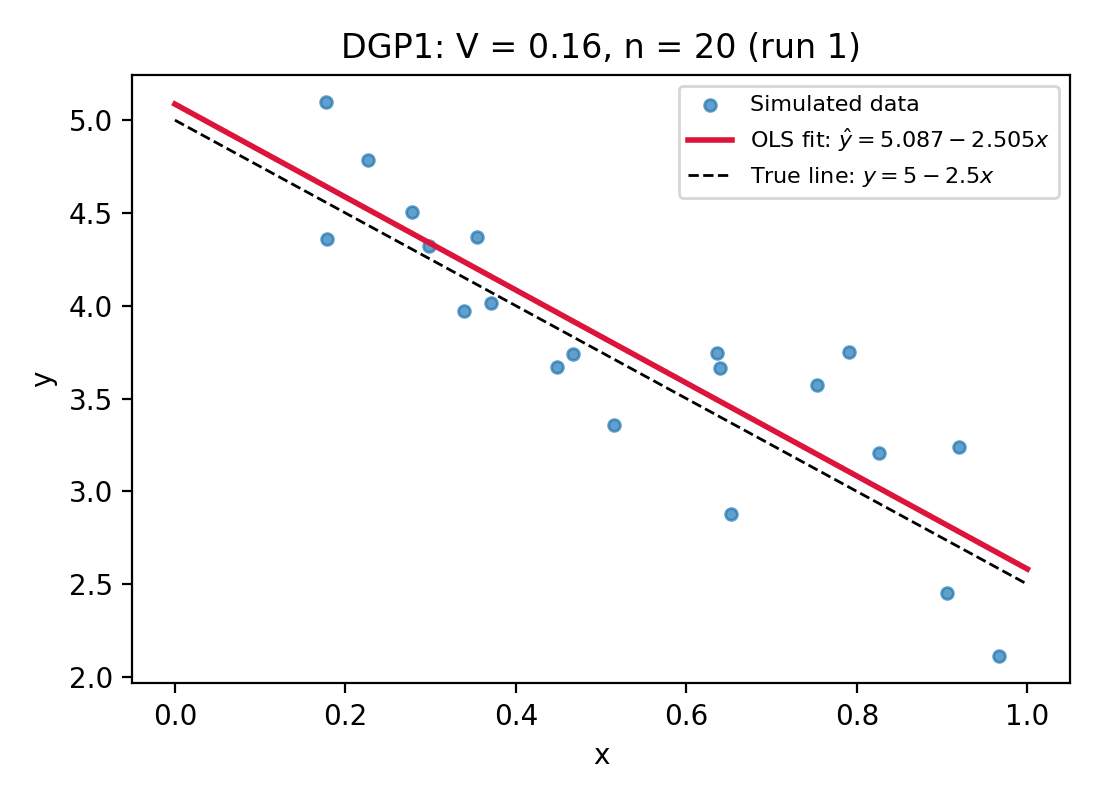
\includegraphics[width=\textwidth]{dgp1_fit.png}\end{subfigure}
  \begin{subfigure}{0.325\textwidth}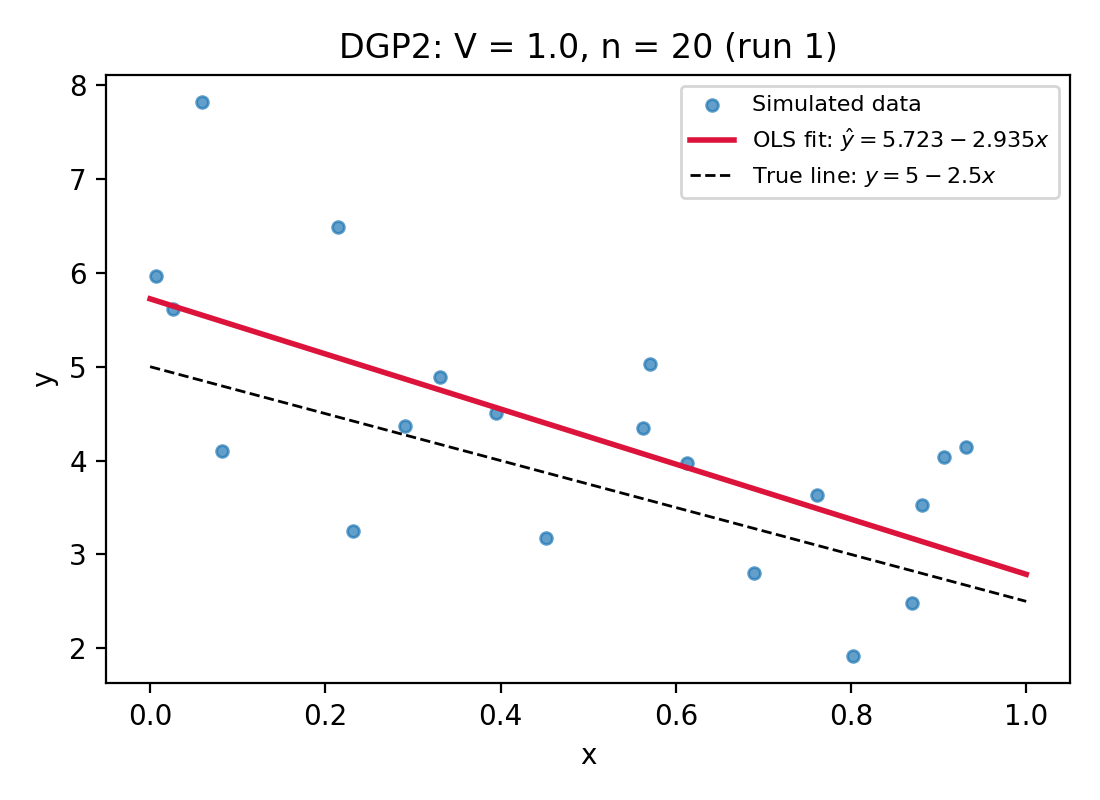
\includegraphics[width=\textwidth]{dgp2_fit.png}\end{subfigure}
  \begin{subfigure}{0.325\textwidth}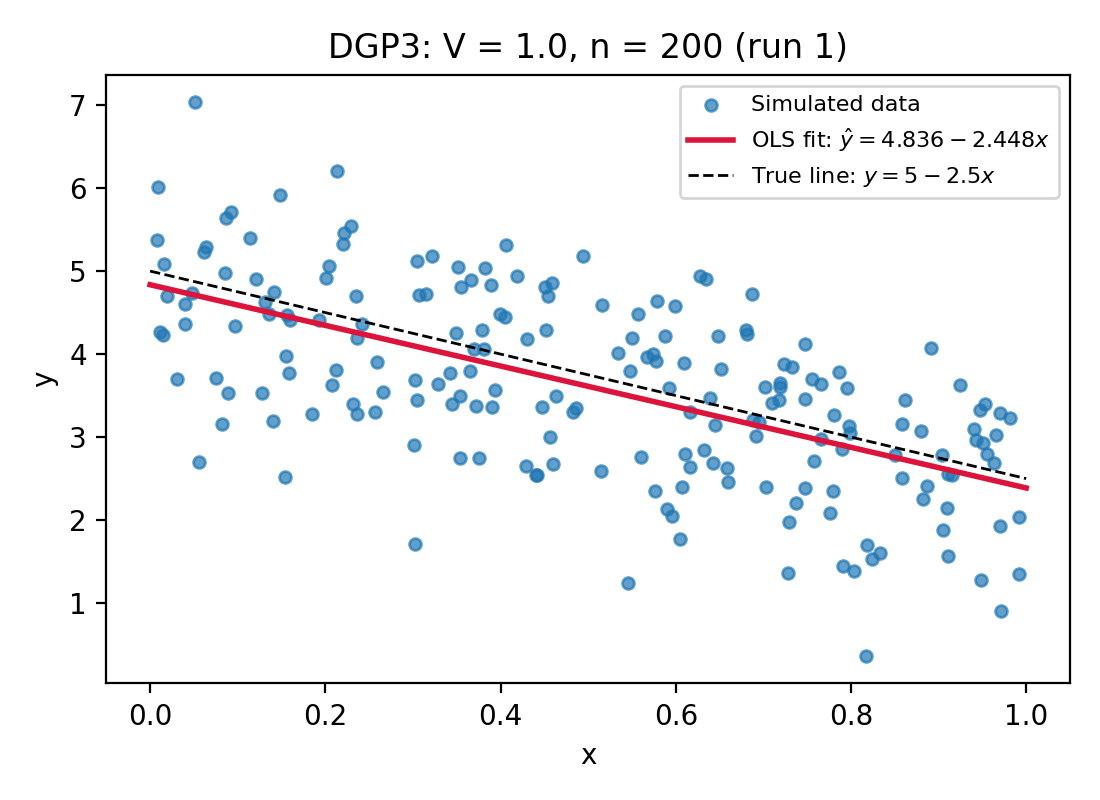
\includegraphics[width=\textwidth]{dgp3_fit.png}\end{subfigure}
  \caption{Data and OLS fit, first run of each DGP. Dashed line: true model $y=5-2.5x$.}
  \label{fig:fits}
\end{figure}

\section*{2. Results}
Table~\ref{tab:res} reports the ten estimates for each design, their average, and their sample standard deviation across runs. Run~1 corresponds to Figure~\ref{fig:fits}. The sample standard deviations use a denominator of $10-1$.

For comparison, the table also gives large-sample approximations to the standard deviations: $\sqrt{4V/n}$ for the intercept and $\sqrt{12V/n}$ for the slope. These follow from $\operatorname{Var}(\hat\beta\mid X)=V(X'X)^{-1}$ and the population moments $E[x]=1/2$ and $E[x^2]=1/3$. They describe the expected pattern of precision, rather than exact finite-sample standard deviations.

\newpage
\begin{table}[H]
\centering
\footnotesize
\setlength{\tabcolsep}{5pt}
\begin{tabular}{lrrrrrr}
\toprule
 & \multicolumn{2}{c}{DGP1} & \multicolumn{2}{c}{DGP2} & \multicolumn{2}{c}{DGP3} \\
Run & $\hat\beta_0$ & $\hat\beta_1$ & $\hat\beta_0$ & $\hat\beta_1$ & $\hat\beta_0$ & $\hat\beta_1$ \\
\midrule
1 & 5.0865 & -2.5045 & 5.7230 & -2.9348 & 4.8357 & -2.4485 \\
2 & 4.7899 & -2.2518 & 4.6799 & -2.2719 & 4.6798 & -2.1085 \\
3 & 4.9072 & -2.4293 & 5.0915 & -2.5309 & 4.7245 & -2.2813 \\
4 & 4.7564 & -2.1248 & 5.0644 & -3.1262 & 5.1651 & -2.8934 \\
5 & 4.9386 & -2.3473 & 4.9944 & -3.0375 & 5.0535 & -2.6810 \\
6 & 4.6632 & -2.1162 & 5.2115 & -2.8415 & 4.8758 & -2.3414 \\
7 & 5.1338 & -2.8707 & 4.8987 & -2.8717 & 5.0708 & -2.5751 \\
8 & 4.9058 & -2.0711 & 4.6316 & -1.7000 & 5.4388 & -3.1286 \\
9 & 4.6653 & -2.1443 & 5.6359 & -3.7015 & 4.7588 & -2.1055 \\
10 & 4.9624 & -2.2975 & 5.2500 & -2.8237 & 5.0194 & -2.3073 \\
\midrule
Mean & 4.8809 & -2.3158 & 5.1181 & -2.7840 & 4.9622 & -2.4871 \\
SD across runs & 0.1616 & 0.2421 & 0.3584 & 0.5333 & 0.2340 & 0.3347 \\
Approximate SD & 0.1789 & 0.3098 & 0.4472 & 0.7746 & 0.1414 & 0.2449 \\
\midrule
True value & 5.0000 & -2.5000 & 5.0000 & -2.5000 & 5.0000 & -2.5000 \\
\bottomrule
\end{tabular}

\caption{OLS estimates over 10 repetitions for each DGP.}
\label{tab:res}
\end{table}

\section*{3. Discussion}
\textbf{Unbiasedness.}
The true intercept is 5 and the true slope is $-2.5$. OLS is unbiased in all three designs because the errors have mean zero and are independent of $x$. This means that, over repeated samples, the estimates are centred on the true values. It does not mean that every estimate, or the average of just ten estimates, equals the truth.

\textbf{More noise: DGP1 versus DGP2.}
Both designs use 20 observations. Increasing the error variance from 0.16 to 1 makes the points more scattered around the true line and the estimates less precise. In our ten runs, the standard deviation of the slope estimates rises from 0.24 to 0.53. The estimates therefore vary more from one sample to another.

\textbf{More observations: DGP2 versus DGP3.}
Both designs have error variance 1, but DGP3 uses 200 observations instead of 20. The individual points are still noisy, yet the larger sample helps estimate the line more precisely. The standard deviation of the slope estimates falls from 0.53 to 0.33, and the average slope, $-2.4871$, is close to the true value of $-2.5$.

\textbf{Why precision changes.}
Holding the regressors fixed, the variance of the OLS estimates is proportional to the error variance. More noise therefore makes the estimates less precise. A larger sample provides more information about the line, reducing sampling variability. The approximate standard deviations in Table~1 describe this expected pattern; they are large-sample approximations, not exact values for these particular samples.

\textbf{Interpreting ten runs.}
The averages and standard deviations in Table~1 are based on only ten repetitions, so they also depend on chance. For example, the DGP1 average slope is $-2.3158$, even though OLS is unbiased. DGP3 happens to give the closest average in this simulation, but that ranking is not guaranteed in every set of ten runs. The main finding is that lower error variance and a larger sample improve precision, while the model assumptions imply unbiasedness in every design.
\end{document}
